\documentclass[aspectratio=169]{beamer}

\usetheme{Boadilla}
\usefonttheme{professionalfonts}
\setbeamertemplate{navigation symbols}{}
\setbeamertemplate{itemize items}[circle]
\setbeamertemplate{enumerate items}[default]
\setbeamertemplate{headline}{}

\usepackage[utf8]{inputenc}
\usepackage[T1]{fontenc}
\usepackage{lmodern}
\usepackage{amsmath}
\usepackage{booktabs}
\usepackage{tabularx}
\usepackage{array}
\usepackage{hyperref}
\usepackage[strings]{underscore}
\usepackage{listings}
\usepackage{tikz}
\usetikzlibrary{arrows.meta,positioning,fit,calc,shapes.geometric}
\usepackage{xcolor}

\definecolor{courseblue}{HTML}{12355B}
\definecolor{coursegold}{HTML}{C98A2E}
\definecolor{courseice}{HTML}{EEF3F8}
\definecolor{coursegreen}{HTML}{2F6B4F}
\definecolor{coursegray}{HTML}{4B5563}
\definecolor{codebg}{HTML}{F7F9FC}
\definecolor{codecomment}{HTML}{5E6C84}
\definecolor{codestring}{HTML}{0B6E4F}

\setbeamercolor{palette primary}{bg=courseblue,fg=white}
\setbeamercolor{palette secondary}{bg=coursegold,fg=white}
\setbeamercolor{palette tertiary}{bg=courseblue,fg=white}
\setbeamercolor{palette quaternary}{bg=coursegold,fg=white}
\setbeamercolor{structure}{fg=courseblue}
\setbeamercolor{frametitle}{bg=courseice,fg=courseblue}
\setbeamercolor{title}{fg=courseblue}
\setbeamercolor{block title}{bg=courseblue,fg=white}
\setbeamercolor{block body}{bg=courseice,fg=black}
\setbeamercolor{normal text}{fg=black,bg=white}
\setbeamercolor{alerted text}{fg=coursegold}

\setbeamerfont{footline}{size=\scriptsize}

\setbeamertemplate{footline}{
  \leavevmode
  \hbox{
    \begin{beamercolorbox}[wd=.33\paperwidth,ht=2.8ex,dp=1.2ex,leftskip=0.8em]{palette primary}%
      University of Trieste
    \end{beamercolorbox}%
    \begin{beamercolorbox}[wd=.49\paperwidth,ht=2.8ex,dp=1.2ex,center]{palette tertiary}%
      \coursename{} \textbar{} \coursecode
    \end{beamercolorbox}%
    \begin{beamercolorbox}[wd=.18\paperwidth,ht=2.8ex,dp=1.2ex,rightskip=0.8em plus1fil]{palette secondary}%
      \insertframenumber{} / \inserttotalframenumber
    \end{beamercolorbox}%
  }
}

\hypersetup{
  colorlinks=true,
  linkcolor=courseblue,
  urlcolor=coursegreen
}

\lstdefinestyle{coursepython}{
  language=Python,
  basicstyle=\ttfamily\footnotesize,
  keywordstyle=\color{courseblue}\bfseries,
  commentstyle=\color{codecomment}\itshape,
  stringstyle=\color{codestring},
  showstringspaces=false,
  columns=fullflexible,
  keepspaces=true,
  frame=single,
  framerule=0.6pt,
  rulecolor=\color{courseblue},
  backgroundcolor=\color{codebg},
  xleftmargin=0.4em,
  xrightmargin=0.4em,
  aboveskip=0.4em,
  belowskip=0.2em
}

\newcommand{\coursename}{Data-driven Systems Engineering}
\newcommand{\coursecode}{440MI / 305SM}
\newcommand{\coursefooter}{}

\newcommand{\learninggoals}[1]{
  \begin{block}{Learning goals}
  #1
  \end{block}
}

\newcommand{\repoactivity}[1]{
  \begin{block}{Repo activity}
  #1
  \end{block}
}

\newcommand{\readinglist}[1]{
  \begin{block}{Papers and materials}
  {\footnotesize #1}
  \end{block}
}

\newcommand{\coursecontextframe}[5]{
  \begin{frame}{Course Map and Running Cases}
  \centering
  \begin{tikzpicture}[node distance=0.28cm]
  \node[flowbox, minimum width=1.45cm, minimum height=0.8cm] (problem) {\scriptsize Problem};
  \node[flowbox, minimum width=1.45cm, minimum height=0.8cm, right=of problem] (data) {\scriptsize Data};
  \node[flowbox, minimum width=1.45cm, minimum height=0.8cm, right=of data] (features) {\scriptsize Features};
  \node[flowbox, minimum width=1.45cm, minimum height=0.8cm, right=of features] (model) {\scriptsize Model};
  \node[flowbox, minimum width=1.45cm, minimum height=0.8cm, right=of model] (interface) {\scriptsize Interface};
  \node[flowbox, minimum width=1.45cm, minimum height=0.8cm, right=of interface] (delivery) {\scriptsize Delivery};
  \node[flowbox, minimum width=1.45cm, minimum height=0.8cm, right=of delivery] (monitor) {\scriptsize Monitor};
  \node[accentbox, minimum width=1.6cm, minimum height=0.8cm, right=of monitor] (evolution) {\scriptsize Evolution};
  \foreach \a/\b in {problem/data,data/features,features/model,model/interface,interface/delivery,delivery/monitor,monitor/evolution} {
    \draw[arrow] (\a) -- (\b);
  }
  \end{tikzpicture}

  \vspace{0.5em}
  \begin{block}{Today in the course}
  \textbf{Focus:} #1

  \textbf{Bridge:} #2
  \end{block}

  \begin{columns}[T]
  \column{0.48\textwidth}
  \begin{block}{Fraud case}
  {\footnotesize #3}
  \end{block}
  \column{0.48\textwidth}
  \begin{block}{Pasteurization case}
  {\footnotesize #4}
  \end{block}
  \end{columns}

  \vspace{0.3em}
  {\footnotesize \textbf{Course thread:} #5}
  \coursefooter
  \end{frame}
}

\newcommand{\classclosingframe}[4]{
  \begin{frame}{From This Class to the Next}
  \begin{block}{What stays with us}
  #1
  \end{block}

  \begin{columns}[T]
  \column{0.48\textwidth}
  \begin{block}{Project use}
  {\footnotesize #2}
  \end{block}
  \column{0.48\textwidth}
  \begin{block}{Next connection}
  {\footnotesize #3}
  \end{block}
  \end{columns}

  \vspace{0.3em}
  {\footnotesize \textbf{Course thread:} #4}
  \coursefooter
  \end{frame}
}

\tikzset{
  flowbox/.style={
    rounded corners=3pt,
    draw=courseblue,
    fill=courseice,
    very thick,
    minimum width=2.2cm,
    minimum height=0.9cm,
    align=center,
    font=\small
  },
  accentbox/.style={
    rounded corners=3pt,
    draw=coursegold,
    fill=coursegold!15,
    very thick,
    minimum width=2.2cm,
    minimum height=0.9cm,
    align=center,
    font=\small
  },
  arrow/.style={
    -{Latex[length=2.5mm,width=2mm]},
    thick,
    draw=courseblue
  }
}

% Visual layer on top of common.tex: tiles, icons, a progress-strip section divider, and a footer
% strip that defines the concepts appearing for the first time on each slide.
% Same look as the Class 20 deck. Load with:  \documentclass[aspectratio=169]{beamer}

\usetheme{Boadilla}
\usefonttheme{professionalfonts}
\setbeamertemplate{navigation symbols}{}
\setbeamertemplate{itemize items}[circle]
\setbeamertemplate{enumerate items}[default]
\setbeamertemplate{headline}{}

\usepackage[utf8]{inputenc}
\usepackage[T1]{fontenc}
\usepackage{lmodern}
\usepackage{amsmath}
\usepackage{booktabs}
\usepackage{tabularx}
\usepackage{array}
\usepackage{hyperref}
\usepackage[strings]{underscore}
\usepackage{listings}
\usepackage{tikz}
\usetikzlibrary{arrows.meta,positioning,fit,calc,shapes.geometric}
\usepackage{xcolor}

\definecolor{courseblue}{HTML}{12355B}
\definecolor{coursegold}{HTML}{C98A2E}
\definecolor{courseice}{HTML}{EEF3F8}
\definecolor{coursegreen}{HTML}{2F6B4F}
\definecolor{coursegray}{HTML}{4B5563}
\definecolor{codebg}{HTML}{F7F9FC}
\definecolor{codecomment}{HTML}{5E6C84}
\definecolor{codestring}{HTML}{0B6E4F}

\setbeamercolor{palette primary}{bg=courseblue,fg=white}
\setbeamercolor{palette secondary}{bg=coursegold,fg=white}
\setbeamercolor{palette tertiary}{bg=courseblue,fg=white}
\setbeamercolor{palette quaternary}{bg=coursegold,fg=white}
\setbeamercolor{structure}{fg=courseblue}
\setbeamercolor{frametitle}{bg=courseice,fg=courseblue}
\setbeamercolor{title}{fg=courseblue}
\setbeamercolor{block title}{bg=courseblue,fg=white}
\setbeamercolor{block body}{bg=courseice,fg=black}
\setbeamercolor{normal text}{fg=black,bg=white}
\setbeamercolor{alerted text}{fg=coursegold}

\setbeamerfont{footline}{size=\scriptsize}

\setbeamertemplate{footline}{
  \leavevmode
  \hbox{
    \begin{beamercolorbox}[wd=.33\paperwidth,ht=2.8ex,dp=1.2ex,leftskip=0.8em]{palette primary}%
      University of Trieste
    \end{beamercolorbox}%
    \begin{beamercolorbox}[wd=.49\paperwidth,ht=2.8ex,dp=1.2ex,center]{palette tertiary}%
      \coursename{} \textbar{} \coursecode
    \end{beamercolorbox}%
    \begin{beamercolorbox}[wd=.18\paperwidth,ht=2.8ex,dp=1.2ex,rightskip=0.8em plus1fil]{palette secondary}%
      \insertframenumber{} / \inserttotalframenumber
    \end{beamercolorbox}%
  }
}

\hypersetup{
  colorlinks=true,
  linkcolor=courseblue,
  urlcolor=coursegreen
}

\lstdefinestyle{coursepython}{
  language=Python,
  basicstyle=\ttfamily\footnotesize,
  keywordstyle=\color{courseblue}\bfseries,
  commentstyle=\color{codecomment}\itshape,
  stringstyle=\color{codestring},
  showstringspaces=false,
  columns=fullflexible,
  keepspaces=true,
  frame=single,
  framerule=0.6pt,
  rulecolor=\color{courseblue},
  backgroundcolor=\color{codebg},
  xleftmargin=0.4em,
  xrightmargin=0.4em,
  aboveskip=0.4em,
  belowskip=0.2em
}

\newcommand{\coursename}{Data-driven Systems Engineering}
\newcommand{\coursecode}{440MI / 305SM}
\newcommand{\coursefooter}{}

\newcommand{\learninggoals}[1]{
  \begin{block}{Learning goals}
  #1
  \end{block}
}

\newcommand{\repoactivity}[1]{
  \begin{block}{Repo activity}
  #1
  \end{block}
}

\newcommand{\readinglist}[1]{
  \begin{block}{Papers and materials}
  {\footnotesize #1}
  \end{block}
}

\newcommand{\coursecontextframe}[5]{
  \begin{frame}{Course Map and Running Cases}
  \centering
  \begin{tikzpicture}[node distance=0.28cm]
  \node[flowbox, minimum width=1.45cm, minimum height=0.8cm] (problem) {\scriptsize Problem};
  \node[flowbox, minimum width=1.45cm, minimum height=0.8cm, right=of problem] (data) {\scriptsize Data};
  \node[flowbox, minimum width=1.45cm, minimum height=0.8cm, right=of data] (features) {\scriptsize Features};
  \node[flowbox, minimum width=1.45cm, minimum height=0.8cm, right=of features] (model) {\scriptsize Model};
  \node[flowbox, minimum width=1.45cm, minimum height=0.8cm, right=of model] (interface) {\scriptsize Interface};
  \node[flowbox, minimum width=1.45cm, minimum height=0.8cm, right=of interface] (delivery) {\scriptsize Delivery};
  \node[flowbox, minimum width=1.45cm, minimum height=0.8cm, right=of delivery] (monitor) {\scriptsize Monitor};
  \node[accentbox, minimum width=1.6cm, minimum height=0.8cm, right=of monitor] (evolution) {\scriptsize Evolution};
  \foreach \a/\b in {problem/data,data/features,features/model,model/interface,interface/delivery,delivery/monitor,monitor/evolution} {
    \draw[arrow] (\a) -- (\b);
  }
  \end{tikzpicture}

  \vspace{0.5em}
  \begin{block}{Today in the course}
  \textbf{Focus:} #1

  \textbf{Bridge:} #2
  \end{block}

  \begin{columns}[T]
  \column{0.48\textwidth}
  \begin{block}{Fraud case}
  {\footnotesize #3}
  \end{block}
  \column{0.48\textwidth}
  \begin{block}{Pasteurization case}
  {\footnotesize #4}
  \end{block}
  \end{columns}

  \vspace{0.3em}
  {\footnotesize \textbf{Course thread:} #5}
  \coursefooter
  \end{frame}
}

\newcommand{\classclosingframe}[4]{
  \begin{frame}{From This Class to the Next}
  \begin{block}{What stays with us}
  #1
  \end{block}

  \begin{columns}[T]
  \column{0.48\textwidth}
  \begin{block}{Project use}
  {\footnotesize #2}
  \end{block}
  \column{0.48\textwidth}
  \begin{block}{Next connection}
  {\footnotesize #3}
  \end{block}
  \end{columns}

  \vspace{0.3em}
  {\footnotesize \textbf{Course thread:} #4}
  \coursefooter
  \end{frame}
}

\tikzset{
  flowbox/.style={
    rounded corners=3pt,
    draw=courseblue,
    fill=courseice,
    very thick,
    minimum width=2.2cm,
    minimum height=0.9cm,
    align=center,
    font=\small
  },
  accentbox/.style={
    rounded corners=3pt,
    draw=coursegold,
    fill=coursegold!15,
    very thick,
    minimum width=2.2cm,
    minimum height=0.9cm,
    align=center,
    font=\small
  },
  arrow/.style={
    -{Latex[length=2.5mm,width=2mm]},
    thick,
    draw=courseblue
  }
}
  % Visual layer on top of common.tex: tiles, icons, a progress-strip section divider, and a footer
% strip that defines the concepts appearing for the first time on each slide.
% Same look as the Class 20 deck. Load with:  \documentclass[aspectratio=169]{beamer}

\usetheme{Boadilla}
\usefonttheme{professionalfonts}
\setbeamertemplate{navigation symbols}{}
\setbeamertemplate{itemize items}[circle]
\setbeamertemplate{enumerate items}[default]
\setbeamertemplate{headline}{}

\usepackage[utf8]{inputenc}
\usepackage[T1]{fontenc}
\usepackage{lmodern}
\usepackage{amsmath}
\usepackage{booktabs}
\usepackage{tabularx}
\usepackage{array}
\usepackage{hyperref}
\usepackage[strings]{underscore}
\usepackage{listings}
\usepackage{tikz}
\usetikzlibrary{arrows.meta,positioning,fit,calc,shapes.geometric}
\usepackage{xcolor}

\definecolor{courseblue}{HTML}{12355B}
\definecolor{coursegold}{HTML}{C98A2E}
\definecolor{courseice}{HTML}{EEF3F8}
\definecolor{coursegreen}{HTML}{2F6B4F}
\definecolor{coursegray}{HTML}{4B5563}
\definecolor{codebg}{HTML}{F7F9FC}
\definecolor{codecomment}{HTML}{5E6C84}
\definecolor{codestring}{HTML}{0B6E4F}

\setbeamercolor{palette primary}{bg=courseblue,fg=white}
\setbeamercolor{palette secondary}{bg=coursegold,fg=white}
\setbeamercolor{palette tertiary}{bg=courseblue,fg=white}
\setbeamercolor{palette quaternary}{bg=coursegold,fg=white}
\setbeamercolor{structure}{fg=courseblue}
\setbeamercolor{frametitle}{bg=courseice,fg=courseblue}
\setbeamercolor{title}{fg=courseblue}
\setbeamercolor{block title}{bg=courseblue,fg=white}
\setbeamercolor{block body}{bg=courseice,fg=black}
\setbeamercolor{normal text}{fg=black,bg=white}
\setbeamercolor{alerted text}{fg=coursegold}

\setbeamerfont{footline}{size=\scriptsize}

\setbeamertemplate{footline}{
  \leavevmode
  \hbox{
    \begin{beamercolorbox}[wd=.33\paperwidth,ht=2.8ex,dp=1.2ex,leftskip=0.8em]{palette primary}%
      University of Trieste
    \end{beamercolorbox}%
    \begin{beamercolorbox}[wd=.49\paperwidth,ht=2.8ex,dp=1.2ex,center]{palette tertiary}%
      \coursename{} \textbar{} \coursecode
    \end{beamercolorbox}%
    \begin{beamercolorbox}[wd=.18\paperwidth,ht=2.8ex,dp=1.2ex,rightskip=0.8em plus1fil]{palette secondary}%
      \insertframenumber{} / \inserttotalframenumber
    \end{beamercolorbox}%
  }
}

\hypersetup{
  colorlinks=true,
  linkcolor=courseblue,
  urlcolor=coursegreen
}

\lstdefinestyle{coursepython}{
  language=Python,
  basicstyle=\ttfamily\footnotesize,
  keywordstyle=\color{courseblue}\bfseries,
  commentstyle=\color{codecomment}\itshape,
  stringstyle=\color{codestring},
  showstringspaces=false,
  columns=fullflexible,
  keepspaces=true,
  frame=single,
  framerule=0.6pt,
  rulecolor=\color{courseblue},
  backgroundcolor=\color{codebg},
  xleftmargin=0.4em,
  xrightmargin=0.4em,
  aboveskip=0.4em,
  belowskip=0.2em
}

\newcommand{\coursename}{Data-driven Systems Engineering}
\newcommand{\coursecode}{440MI / 305SM}
\newcommand{\coursefooter}{}

\newcommand{\learninggoals}[1]{
  \begin{block}{Learning goals}
  #1
  \end{block}
}

\newcommand{\repoactivity}[1]{
  \begin{block}{Repo activity}
  #1
  \end{block}
}

\newcommand{\readinglist}[1]{
  \begin{block}{Papers and materials}
  {\footnotesize #1}
  \end{block}
}

\newcommand{\coursecontextframe}[5]{
  \begin{frame}{Course Map and Running Cases}
  \centering
  \begin{tikzpicture}[node distance=0.28cm]
  \node[flowbox, minimum width=1.45cm, minimum height=0.8cm] (problem) {\scriptsize Problem};
  \node[flowbox, minimum width=1.45cm, minimum height=0.8cm, right=of problem] (data) {\scriptsize Data};
  \node[flowbox, minimum width=1.45cm, minimum height=0.8cm, right=of data] (features) {\scriptsize Features};
  \node[flowbox, minimum width=1.45cm, minimum height=0.8cm, right=of features] (model) {\scriptsize Model};
  \node[flowbox, minimum width=1.45cm, minimum height=0.8cm, right=of model] (interface) {\scriptsize Interface};
  \node[flowbox, minimum width=1.45cm, minimum height=0.8cm, right=of interface] (delivery) {\scriptsize Delivery};
  \node[flowbox, minimum width=1.45cm, minimum height=0.8cm, right=of delivery] (monitor) {\scriptsize Monitor};
  \node[accentbox, minimum width=1.6cm, minimum height=0.8cm, right=of monitor] (evolution) {\scriptsize Evolution};
  \foreach \a/\b in {problem/data,data/features,features/model,model/interface,interface/delivery,delivery/monitor,monitor/evolution} {
    \draw[arrow] (\a) -- (\b);
  }
  \end{tikzpicture}

  \vspace{0.5em}
  \begin{block}{Today in the course}
  \textbf{Focus:} #1

  \textbf{Bridge:} #2
  \end{block}

  \begin{columns}[T]
  \column{0.48\textwidth}
  \begin{block}{Fraud case}
  {\footnotesize #3}
  \end{block}
  \column{0.48\textwidth}
  \begin{block}{Pasteurization case}
  {\footnotesize #4}
  \end{block}
  \end{columns}

  \vspace{0.3em}
  {\footnotesize \textbf{Course thread:} #5}
  \coursefooter
  \end{frame}
}

\newcommand{\classclosingframe}[4]{
  \begin{frame}{From This Class to the Next}
  \begin{block}{What stays with us}
  #1
  \end{block}

  \begin{columns}[T]
  \column{0.48\textwidth}
  \begin{block}{Project use}
  {\footnotesize #2}
  \end{block}
  \column{0.48\textwidth}
  \begin{block}{Next connection}
  {\footnotesize #3}
  \end{block}
  \end{columns}

  \vspace{0.3em}
  {\footnotesize \textbf{Course thread:} #4}
  \coursefooter
  \end{frame}
}

\tikzset{
  flowbox/.style={
    rounded corners=3pt,
    draw=courseblue,
    fill=courseice,
    very thick,
    minimum width=2.2cm,
    minimum height=0.9cm,
    align=center,
    font=\small
  },
  accentbox/.style={
    rounded corners=3pt,
    draw=coursegold,
    fill=coursegold!15,
    very thick,
    minimum width=2.2cm,
    minimum height=0.9cm,
    align=center,
    font=\small
  },
  arrow/.style={
    -{Latex[length=2.5mm,width=2mm]},
    thick,
    draw=courseblue
  }
}
  % Visual layer on top of common.tex: tiles, icons, a progress-strip section divider, and a footer
% strip that defines the concepts appearing for the first time on each slide.
% Same look as the Class 20 deck. Load with:  \input{common}  \input{common_visual}
%
% Before the first \sectiondivider, a deck must define
%   \sectioncount   the number of sections, e.g. 4
%   \sectionlabels  a \foreach list of number/label pairs, e.g. 1/Need,2/Testable,3/Manage,4/Practice
% Icons come from the fontawesome5 package (Font Awesome 5 Free), e.g. \faIcon{robot}.

\usepackage{colortbl}
\usepackage{fontawesome5}
\usetikzlibrary{backgrounds}

% Slides read better without automatic hyphenation.
\hyphenpenalty=10000
\exhyphenpenalty=10000

\definecolor{coursered}{HTML}{A23B2A}
\newcommand{\goldink}{\color{coursegold!65!black}}

\tikzset{
  tile/.style={rounded corners=4pt, fill=courseice, draw=none, align=center, font=\footnotesize, inner sep=5pt},
  tileblue/.style={tile, fill=white, draw=courseblue!55, thick},
  tilegold/.style={tile, fill=coursegold!14, draw=coursegold, thick},
  tilegreen/.style={tile, fill=coursegreen!10, draw=coursegreen!70, thick},
  tilered/.style={tile, fill=coursered!8, draw=coursered!70, thick},
  tilegray/.style={tile, fill=white, draw=coursegray!55, thick, dashed},
  tag/.style={rounded corners=2pt, fill=coursegold, text=white, font=\bfseries\tiny, inner sep=2.5pt},
  chip/.style={rounded corners=3pt, fill=courseblue, text=white, font=\footnotesize\bfseries, align=center, inner sep=4pt},
  note/.style={font=\scriptsize, text=coursegray, align=left},
  arrowgold/.style={-{Latex[length=2.5mm,width=2mm]}, thick, draw=coursegold},
  arrowred/.style={-{Latex[length=2.5mm,width=2mm]}, thick, draw=coursered},
  arrowgreen/.style={-{Latex[length=2.5mm,width=2mm]}, thick, draw=coursegreen},
  arrowgray/.style={-{Latex[length=2mm,width=1.6mm]}, thick, draw=coursegray!70},
}

% A round icon badge, drawn inside a tikzpicture: x y colour icon
\newcommand{\badge}[4]{%
  \node[circle, fill=#3, text=white, minimum size=0.85cm, inner sep=0pt] at (#1,#2) {\large\faIcon{#4}};
}

% Inline tags for the kind of requirement.
\newcommand{\Ftag}{\colorbox{courseblue}{\color{white}\bfseries\scriptsize\ \ F\ \ }}
\newcommand{\NFtag}{\colorbox{coursegold}{\color{white}\bfseries\scriptsize\ NF\ }}
\newcommand{\Dtag}{\colorbox{coursegreen}{\color{white}\bfseries\scriptsize\ \ D\ \ }}
\newcommand{\MLtag}{\colorbox{coursered}{\color{white}\bfseries\scriptsize\ ML\ }}

% Footer: a strip with the concepts that appear for the first time on the slide, above the
% usual bar. The bar total counts only the main lecture; a backup slide is numbered separately.
\makeatletter
\def\conceptstext{}
\def\currentsectionname{}
\setbeamercolor{conceptbar}{bg=coursegold!12,fg=black}
\newcommand{\cterm}[2]{{\bfseries\color{courseblue}#1:}\ #2\hspace{0.8em}}
\newcommand{\newtag}{\colorbox{coursegold}{\color{white}\bfseries\tiny\ NEW\ }\hspace{0.6em}}
\setbeamertemplate{footline}{
  \leavevmode
  \vbox{%
    \ifx\conceptstext\empty\else
      \hbox{\color{coursegold}\rule{\paperwidth}{0.8pt}}%
      \hbox{\begin{beamercolorbox}[wd=\paperwidth,leftskip=0.5cm,rightskip=0.5cm,sep=3pt]{conceptbar}\scriptsize\newtag\conceptstext\end{beamercolorbox}}%
    \fi
    \hbox{%
      \begin{beamercolorbox}[wd=.33\paperwidth,ht=2.8ex,dp=1.2ex,leftskip=0.8em]{palette primary}%
        \ifbeamer@inappendix Backup\else\ifnum\value{section}>0 \arabic{section}\ \textbar\ \currentsectionname\else University of Trieste\fi\fi
      \end{beamercolorbox}%
      \begin{beamercolorbox}[wd=.49\paperwidth,ht=2.8ex,dp=1.2ex,center]{palette tertiary}%
        \coursename{} \textbar{} \coursecode
      \end{beamercolorbox}%
      \begin{beamercolorbox}[wd=.18\paperwidth,ht=2.8ex,dp=1.2ex,right,rightskip=0.8em]{palette secondary}%
        \ifbeamer@inappendix Backup \insertframenumberinappendix\else\insertframenumber{} / \insertmainframenumber\fi
      \end{beamercolorbox}%
    }}}
\makeatother
\newenvironment{cframe}[2]{\gdef\conceptstext{#2}\begin{frame}{#1}}{\end{frame}\gdef\conceptstext{}}

% Section divider: progress strip, recap of the previous part, and the roadmap of the next one.
% Arguments: number, title, icon, previously, items.
\newcommand{\sectiondivider}[5]{%
  \section{#2}\gdef\currentsectionname{#2}
  \begin{frame}
  \centering
  \begin{tikzpicture}
  \pgfmathsetmacro{\chipw}{13.6/\sectioncount}
  \foreach \i/\lab in \sectionlabels {
    \ifnum\i<#1 \def\chipfill{courseblue!22}\def\chiptext{courseblue}\else
    \ifnum\i=#1 \def\chipfill{courseblue}\def\chiptext{white}\else
    \def\chipfill{courseice}\def\chiptext{coursegray}\fi\fi
    \node[rounded corners=3pt, minimum width={(\chipw-0.1)*1cm}, minimum height=0.6cm, font=\scriptsize\bfseries, fill=\chipfill, text=\chiptext] at ({\chipw/2+(\i-1)*\chipw},0) {\i\ \lab};
  }
  \node[circle, fill=courseblue, text=white, font=\Huge\bfseries, minimum size=1.7cm, inner sep=0] at (1.0,-1.7) {#1};
  \node[anchor=west, font=\huge\bfseries, text=courseblue, text width=8.8cm, align=left] at (2.2,-1.7) {#2};
  \node[circle, fill=coursegold!16, draw=coursegold, thick, text=coursegold!75!black, font=\fontsize{26}{26}\selectfont, minimum size=1.9cm, inner sep=0] at (12.6,-1.7) {\faIcon{#3}};
  \ifx\relax#4\relax\else
    \node[anchor=north west, font=\small\itshape, text=coursegray, text width=13.2cm, align=left] at (0.1,-2.95) {Previously: #4};
  \fi
  \node[anchor=north west, font=\footnotesize\bfseries, text=coursegold!65!black] at (0.1,-3.95) {IN THIS PART};
  \node[anchor=north west, font=\small, text width=13.2cm, align=left] at (0.1,-4.35) {#5};
  \end{tikzpicture}
  \end{frame}
}

%
% Before the first \sectiondivider, a deck must define
%   \sectioncount   the number of sections, e.g. 4
%   \sectionlabels  a \foreach list of number/label pairs, e.g. 1/Need,2/Testable,3/Manage,4/Practice
% Icons come from the fontawesome5 package (Font Awesome 5 Free), e.g. \faIcon{robot}.

\usepackage{colortbl}
\usepackage{fontawesome5}
\usetikzlibrary{backgrounds}

% Slides read better without automatic hyphenation.
\hyphenpenalty=10000
\exhyphenpenalty=10000

\definecolor{coursered}{HTML}{A23B2A}
\newcommand{\goldink}{\color{coursegold!65!black}}

\tikzset{
  tile/.style={rounded corners=4pt, fill=courseice, draw=none, align=center, font=\footnotesize, inner sep=5pt},
  tileblue/.style={tile, fill=white, draw=courseblue!55, thick},
  tilegold/.style={tile, fill=coursegold!14, draw=coursegold, thick},
  tilegreen/.style={tile, fill=coursegreen!10, draw=coursegreen!70, thick},
  tilered/.style={tile, fill=coursered!8, draw=coursered!70, thick},
  tilegray/.style={tile, fill=white, draw=coursegray!55, thick, dashed},
  tag/.style={rounded corners=2pt, fill=coursegold, text=white, font=\bfseries\tiny, inner sep=2.5pt},
  chip/.style={rounded corners=3pt, fill=courseblue, text=white, font=\footnotesize\bfseries, align=center, inner sep=4pt},
  note/.style={font=\scriptsize, text=coursegray, align=left},
  arrowgold/.style={-{Latex[length=2.5mm,width=2mm]}, thick, draw=coursegold},
  arrowred/.style={-{Latex[length=2.5mm,width=2mm]}, thick, draw=coursered},
  arrowgreen/.style={-{Latex[length=2.5mm,width=2mm]}, thick, draw=coursegreen},
  arrowgray/.style={-{Latex[length=2mm,width=1.6mm]}, thick, draw=coursegray!70},
}

% A round icon badge, drawn inside a tikzpicture: x y colour icon
\newcommand{\badge}[4]{%
  \node[circle, fill=#3, text=white, minimum size=0.85cm, inner sep=0pt] at (#1,#2) {\large\faIcon{#4}};
}

% Inline tags for the kind of requirement.
\newcommand{\Ftag}{\colorbox{courseblue}{\color{white}\bfseries\scriptsize\ \ F\ \ }}
\newcommand{\NFtag}{\colorbox{coursegold}{\color{white}\bfseries\scriptsize\ NF\ }}
\newcommand{\Dtag}{\colorbox{coursegreen}{\color{white}\bfseries\scriptsize\ \ D\ \ }}
\newcommand{\MLtag}{\colorbox{coursered}{\color{white}\bfseries\scriptsize\ ML\ }}

% Footer: a strip with the concepts that appear for the first time on the slide, above the
% usual bar. The bar total counts only the main lecture; a backup slide is numbered separately.
\makeatletter
\def\conceptstext{}
\def\currentsectionname{}
\setbeamercolor{conceptbar}{bg=coursegold!12,fg=black}
\newcommand{\cterm}[2]{{\bfseries\color{courseblue}#1:}\ #2\hspace{0.8em}}
\newcommand{\newtag}{\colorbox{coursegold}{\color{white}\bfseries\tiny\ NEW\ }\hspace{0.6em}}
\setbeamertemplate{footline}{
  \leavevmode
  \vbox{%
    \ifx\conceptstext\empty\else
      \hbox{\color{coursegold}\rule{\paperwidth}{0.8pt}}%
      \hbox{\begin{beamercolorbox}[wd=\paperwidth,leftskip=0.5cm,rightskip=0.5cm,sep=3pt]{conceptbar}\scriptsize\newtag\conceptstext\end{beamercolorbox}}%
    \fi
    \hbox{%
      \begin{beamercolorbox}[wd=.33\paperwidth,ht=2.8ex,dp=1.2ex,leftskip=0.8em]{palette primary}%
        \ifbeamer@inappendix Backup\else\ifnum\value{section}>0 \arabic{section}\ \textbar\ \currentsectionname\else University of Trieste\fi\fi
      \end{beamercolorbox}%
      \begin{beamercolorbox}[wd=.49\paperwidth,ht=2.8ex,dp=1.2ex,center]{palette tertiary}%
        \coursename{} \textbar{} \coursecode
      \end{beamercolorbox}%
      \begin{beamercolorbox}[wd=.18\paperwidth,ht=2.8ex,dp=1.2ex,right,rightskip=0.8em]{palette secondary}%
        \ifbeamer@inappendix Backup \insertframenumberinappendix\else\insertframenumber{} / \insertmainframenumber\fi
      \end{beamercolorbox}%
    }}}
\makeatother
\newenvironment{cframe}[2]{\gdef\conceptstext{#2}\begin{frame}{#1}}{\end{frame}\gdef\conceptstext{}}

% Section divider: progress strip, recap of the previous part, and the roadmap of the next one.
% Arguments: number, title, icon, previously, items.
\newcommand{\sectiondivider}[5]{%
  \section{#2}\gdef\currentsectionname{#2}
  \begin{frame}
  \centering
  \begin{tikzpicture}
  \pgfmathsetmacro{\chipw}{13.6/\sectioncount}
  \foreach \i/\lab in \sectionlabels {
    \ifnum\i<#1 \def\chipfill{courseblue!22}\def\chiptext{courseblue}\else
    \ifnum\i=#1 \def\chipfill{courseblue}\def\chiptext{white}\else
    \def\chipfill{courseice}\def\chiptext{coursegray}\fi\fi
    \node[rounded corners=3pt, minimum width={(\chipw-0.1)*1cm}, minimum height=0.6cm, font=\scriptsize\bfseries, fill=\chipfill, text=\chiptext] at ({\chipw/2+(\i-1)*\chipw},0) {\i\ \lab};
  }
  \node[circle, fill=courseblue, text=white, font=\Huge\bfseries, minimum size=1.7cm, inner sep=0] at (1.0,-1.7) {#1};
  \node[anchor=west, font=\huge\bfseries, text=courseblue, text width=8.8cm, align=left] at (2.2,-1.7) {#2};
  \node[circle, fill=coursegold!16, draw=coursegold, thick, text=coursegold!75!black, font=\fontsize{26}{26}\selectfont, minimum size=1.9cm, inner sep=0] at (12.6,-1.7) {\faIcon{#3}};
  \ifx\relax#4\relax\else
    \node[anchor=north west, font=\small\itshape, text=coursegray, text width=13.2cm, align=left] at (0.1,-2.95) {Previously: #4};
  \fi
  \node[anchor=north west, font=\footnotesize\bfseries, text=coursegold!65!black] at (0.1,-3.95) {IN THIS PART};
  \node[anchor=north west, font=\small, text width=13.2cm, align=left] at (0.1,-4.35) {#5};
  \end{tikzpicture}
  \end{frame}
}

%
% Before the first \sectiondivider, a deck must define
%   \sectioncount   the number of sections, e.g. 4
%   \sectionlabels  a \foreach list of number/label pairs, e.g. 1/Need,2/Testable,3/Manage,4/Practice
% Icons come from the fontawesome5 package (Font Awesome 5 Free), e.g. \faIcon{robot}.

\usepackage{colortbl}
\usepackage{fontawesome5}
\usetikzlibrary{backgrounds}

% Slides read better without automatic hyphenation.
\hyphenpenalty=10000
\exhyphenpenalty=10000

\definecolor{coursered}{HTML}{A23B2A}
\newcommand{\goldink}{\color{coursegold!65!black}}

\tikzset{
  tile/.style={rounded corners=4pt, fill=courseice, draw=none, align=center, font=\footnotesize, inner sep=5pt},
  tileblue/.style={tile, fill=white, draw=courseblue!55, thick},
  tilegold/.style={tile, fill=coursegold!14, draw=coursegold, thick},
  tilegreen/.style={tile, fill=coursegreen!10, draw=coursegreen!70, thick},
  tilered/.style={tile, fill=coursered!8, draw=coursered!70, thick},
  tilegray/.style={tile, fill=white, draw=coursegray!55, thick, dashed},
  tag/.style={rounded corners=2pt, fill=coursegold, text=white, font=\bfseries\tiny, inner sep=2.5pt},
  chip/.style={rounded corners=3pt, fill=courseblue, text=white, font=\footnotesize\bfseries, align=center, inner sep=4pt},
  note/.style={font=\scriptsize, text=coursegray, align=left},
  arrowgold/.style={-{Latex[length=2.5mm,width=2mm]}, thick, draw=coursegold},
  arrowred/.style={-{Latex[length=2.5mm,width=2mm]}, thick, draw=coursered},
  arrowgreen/.style={-{Latex[length=2.5mm,width=2mm]}, thick, draw=coursegreen},
  arrowgray/.style={-{Latex[length=2mm,width=1.6mm]}, thick, draw=coursegray!70},
}

% A round icon badge, drawn inside a tikzpicture: x y colour icon
\newcommand{\badge}[4]{%
  \node[circle, fill=#3, text=white, minimum size=0.85cm, inner sep=0pt] at (#1,#2) {\large\faIcon{#4}};
}

% Inline tags for the kind of requirement.
\newcommand{\Ftag}{\colorbox{courseblue}{\color{white}\bfseries\scriptsize\ \ F\ \ }}
\newcommand{\NFtag}{\colorbox{coursegold}{\color{white}\bfseries\scriptsize\ NF\ }}
\newcommand{\Dtag}{\colorbox{coursegreen}{\color{white}\bfseries\scriptsize\ \ D\ \ }}
\newcommand{\MLtag}{\colorbox{coursered}{\color{white}\bfseries\scriptsize\ ML\ }}

% Footer: a strip with the concepts that appear for the first time on the slide, above the
% usual bar. The bar total counts only the main lecture; a backup slide is numbered separately.
\makeatletter
\def\conceptstext{}
\def\currentsectionname{}
\setbeamercolor{conceptbar}{bg=coursegold!12,fg=black}
\newcommand{\cterm}[2]{{\bfseries\color{courseblue}#1:}\ #2\hspace{0.8em}}
\newcommand{\newtag}{\colorbox{coursegold}{\color{white}\bfseries\tiny\ NEW\ }\hspace{0.6em}}
\setbeamertemplate{footline}{
  \leavevmode
  \vbox{%
    \ifx\conceptstext\empty\else
      \hbox{\color{coursegold}\rule{\paperwidth}{0.8pt}}%
      \hbox{\begin{beamercolorbox}[wd=\paperwidth,leftskip=0.5cm,rightskip=0.5cm,sep=3pt]{conceptbar}\scriptsize\newtag\conceptstext\end{beamercolorbox}}%
    \fi
    \hbox{%
      \begin{beamercolorbox}[wd=.33\paperwidth,ht=2.8ex,dp=1.2ex,leftskip=0.8em]{palette primary}%
        \ifbeamer@inappendix Backup\else\ifnum\value{section}>0 \arabic{section}\ \textbar\ \currentsectionname\else University of Trieste\fi\fi
      \end{beamercolorbox}%
      \begin{beamercolorbox}[wd=.49\paperwidth,ht=2.8ex,dp=1.2ex,center]{palette tertiary}%
        \coursename{} \textbar{} \coursecode
      \end{beamercolorbox}%
      \begin{beamercolorbox}[wd=.18\paperwidth,ht=2.8ex,dp=1.2ex,right,rightskip=0.8em]{palette secondary}%
        \ifbeamer@inappendix Backup \insertframenumberinappendix\else\insertframenumber{} / \insertmainframenumber\fi
      \end{beamercolorbox}%
    }}}
\makeatother
\newenvironment{cframe}[2]{\gdef\conceptstext{#2}\begin{frame}{#1}}{\end{frame}\gdef\conceptstext{}}

% Section divider: progress strip, recap of the previous part, and the roadmap of the next one.
% Arguments: number, title, icon, previously, items.
\newcommand{\sectiondivider}[5]{%
  \section{#2}\gdef\currentsectionname{#2}
  \begin{frame}
  \centering
  \begin{tikzpicture}
  \pgfmathsetmacro{\chipw}{13.6/\sectioncount}
  \foreach \i/\lab in \sectionlabels {
    \ifnum\i<#1 \def\chipfill{courseblue!22}\def\chiptext{courseblue}\else
    \ifnum\i=#1 \def\chipfill{courseblue}\def\chiptext{white}\else
    \def\chipfill{courseice}\def\chiptext{coursegray}\fi\fi
    \node[rounded corners=3pt, minimum width={(\chipw-0.1)*1cm}, minimum height=0.6cm, font=\scriptsize\bfseries, fill=\chipfill, text=\chiptext] at ({\chipw/2+(\i-1)*\chipw},0) {\i\ \lab};
  }
  \node[circle, fill=courseblue, text=white, font=\Huge\bfseries, minimum size=1.7cm, inner sep=0] at (1.0,-1.7) {#1};
  \node[anchor=west, font=\huge\bfseries, text=courseblue, text width=8.8cm, align=left] at (2.2,-1.7) {#2};
  \node[circle, fill=coursegold!16, draw=coursegold, thick, text=coursegold!75!black, font=\fontsize{26}{26}\selectfont, minimum size=1.9cm, inner sep=0] at (12.6,-1.7) {\faIcon{#3}};
  \ifx\relax#4\relax\else
    \node[anchor=north west, font=\small\itshape, text=coursegray, text width=13.2cm, align=left] at (0.1,-2.95) {Previously: #4};
  \fi
  \node[anchor=north west, font=\footnotesize\bfseries, text=coursegold!65!black] at (0.1,-3.95) {IN THIS PART};
  \node[anchor=north west, font=\small, text width=13.2cm, align=left] at (0.1,-4.35) {#5};
  \end{tikzpicture}
  \end{frame}
}


% Four parts; the progress strip on each divider uses these labels.
\newcommand{\sectioncount}{4}
\newcommand{\sectionlabels}{1/Why MLOps,2/Lifecycle,3/Training,4/Repository}

\title{Class 27: MLOps Foundations and Continuous Training}
\author{\coursename}
\date{}

% ------------------------------------------------------------------ helpers
% A gold strip with a labelled idea: y icon label text
\newcommand{\callout}[4]{%
  \node[tilegold, anchor=north west, minimum width=13.4cm, minimum height=0.8cm, text width=12.6cm, align=left, font=\footnotesize] at (0,#1) {{\bfseries\goldink\faIcon{#2}\ #3}\ #4};
}
% The usual closing idea of a slide
\newcommand{\keyidea}[2]{\callout{#1}{lightbulb}{Key idea.}{#2}}
% A red strip: y icon label text
\newcommand{\warning}[4]{%
  \node[tilered, anchor=north west, minimum width=13.4cm, minimum height=0.8cm, text width=12.6cm, align=left, font=\footnotesize] at (0,#1) {{\bfseries\color{coursered}\faIcon{#2}\ #3}\ #4};
}
% A goal card (6.6 x 1.6): x y style icon title text
\newcommand{\goalcard}[6]{%
  \node[#3, anchor=north west, minimum width=6.6cm, minimum height=1.6cm] at (#1,#2) {};
  \badge{#1+0.65}{#2-0.8}{courseblue}{#4}
  \node[anchor=west, text width=5.2cm, align=left, font=\small\bfseries, text=courseblue] at (#1+1.25,#2-0.28) {#5};
  \node[anchor=north west, text width=5.2cm, align=left, font=\scriptsize, inner sep=0pt] at (#1+1.25,#2-0.5) {#6};
}
% An information tile: x y width height style colour icon title text
\newcommand{\infotile}[9]{%
  \node[#5, anchor=north west, minimum width=#3cm, minimum height=#4cm] at (#1,#2) {};
  \badge{#1+0.55}{#2-0.55}{#6}{#7}
  \node[anchor=west, text width={(#3-1.35)*1cm}, align=left, font=\footnotesize\bfseries, text=courseblue] at (#1+1.05,#2-0.55) {#8};
  \node[anchor=north west, text width={(#3-0.4)*1cm}, align=left, font=\scriptsize, inner sep=0pt] at (#1+0.2,#2-1.0) {#9};
}
% One row of a two-column list: y icon label text
\newcommand{\listrow}[4]{%
  \node[chip, anchor=west, minimum width=4.3cm, minimum height=0.55cm, font=\scriptsize\bfseries, align=left] at (0,#1) {\faIcon{#2}\ #3};
  \node[anchor=west, text width=8.7cm, font=\scriptsize, align=left] at (4.5,#1) {#4};
  \draw[courseice!70!courseblue, line width=0.5pt] (0,#1-0.36) -- (13.4,#1-0.36);
}
% One row of the repository map: y path text stage-colour stage
\newcommand{\reporow}[5]{%
  \node[tile, fill=courseice, anchor=north west, minimum width=4.6cm, minimum height=0.74cm, inner sep=2pt, text width=4.3cm, align=left, font=\ttfamily\scriptsize] at (0,#1) {#2};
  \node[tile, fill=white, draw=courseblue!40, thick, anchor=north west, minimum width=6.3cm, minimum height=0.74cm, inner sep=2pt, text width=5.9cm, align=left, font=\scriptsize] at (4.75,#1) {#3};
  \node[chip, fill=#4, anchor=north west, minimum width=2.15cm, minimum height=0.74cm, font=\scriptsize\bfseries] at (11.25,#1) {#5};
}
\tikzset{fchip/.style={rounded corners=2pt, fill=courseice, draw=courseblue!55, thick, font=\ttfamily\tiny, inner sep=3pt, minimum height=0.36cm}}

\begin{document}

% ------------------------------------------------------------------ title
\frame{\titlepage \coursefooter}

% ------------------------------------------------------------------ roadmap
\begin{cframe}{Roadmap and goals}{\cterm{MLOps}{coordinating the building, release, and operation of ML systems.}\cterm{Lifecycle}{the stages from idea to retirement.}\cterm{Production-ready}{can be rebuilt, run, and supported by someone else.}}
\centering
\begin{tikzpicture}
\foreach \i/\col/\ico/\ttl/\txt in {0/courseblue/bullseye/Why MLOps/{Why ML fails after the notebook, and what maturity changes.}, 1/courseblue/sync-alt/The lifecycle/{Workflow, infrastructure, roles, handoffs, and readiness.}, 2/coursegreen/redo-alt/Continuous training/{Triggers, pipeline stages, gates, and failure modes.}, 3/coursegray/folder-open/Repository/{What exists today, and an honest gap.}} {
  \pgfmathsetmacro{\x}{\i*3.4}
  \node[tile, fill=white, draw=\col, thick, anchor=north west, minimum width=3.2cm, minimum height=2.25cm] at (\x,0) {};
  \node[circle, fill=\col, text=white, minimum size=0.5cm, inner sep=0, font=\small\bfseries] at (\x+0.4,-0.45) {\the\numexpr\i+1\relax};
  \node[anchor=west, text width=1.7cm, align=left, font=\footnotesize\bfseries, text=courseblue, inner sep=0pt] at (\x+0.8,-0.45) {\ttl};
  \node[text=\col!70, font=\Large] at (\x+2.8,-0.45) {\faIcon{\ico}};
  \node[anchor=north west, text width=2.8cm, align=left, font=\scriptsize, inner sep=0pt] at (\x+0.2,-1.0) {\txt};
}
\node[anchor=west, font=\tiny\bfseries, text=coursegold!65!black] at (0,-2.55) {WHAT YOU WILL BE ABLE TO DO};
\foreach \x/\y/\ico/\t in {0/-2.7/project-diagram/{Define MLOps as model development joined to operational discipline.}, 6.8/-2.7/users/{Map the roles and handoffs of production ML.}, 0/-3.45/clipboard-check/{Judge whether a project is production-ready or only demo-ready.}, 6.8/-3.45/balance-scale/{Separate what DevOps covers from what MLOps adds.}, 0/-4.2/redo-alt/{Describe a continuous training pipeline and the gates in it.}, 6.8/-4.2/hand-pointer/{Choose retraining triggers; separate retraining from deployment.}} {
  \node[circle, fill=courseblue, text=white, minimum size=0.45cm, inner sep=0, font=\scriptsize] at (\x+0.3,\y-0.3) {\faIcon{\ico}};
  \node[anchor=west, text width=5.8cm, align=left, font=\scriptsize, inner sep=0pt] at (\x+0.7,\y-0.3) {\t};
}
\end{tikzpicture}
\coursefooter
\end{cframe}

% ------------------------------------------------------------------ goals
% ------------------------------------------------------------------ course context
\begin{cframe}{Where this class sits in the course}{\cterm{Running case}{one of two examples, fraud scoring and pasteurization monitoring, that return in every class.}}
\centering
\begin{tikzpicture}
\foreach \i/\lab/\bg/\fg in {0/Problem/courseice/coursegray, 1/Data/courseice/coursegray, 2/Features/courseice/coursegray, 3/Model/courseice/coursegray, 4/Interface/courseice/coursegray, 5/Delivery/courseblue/white, 6/Monitor/courseblue/white, 7/Evolution/courseblue/white} {
  \pgfmathsetmacro{\x}{\i*1.68}
  \node[rounded corners=3pt, fill=\bg, text=\fg, anchor=north west, minimum width=1.55cm, minimum height=0.6cm, font=\scriptsize\bfseries] at (\x,0) {\lab};
}
\node[tilegold, anchor=north west, minimum width=6.6cm, minimum height=1.3cm, text width=6.2cm, align=left] at (0,-0.9) {{\bfseries\goldink\faIcon{bullseye}\ Focus.} Operational ownership across the ML lifecycle, including automated retraining.};
\node[tileblue, anchor=north west, minimum width=6.6cm, minimum height=1.3cm, text width=6.2cm, align=left] at (6.8,-0.9) {{\bfseries\color{courseblue}\faIcon{link}\ Bridge.} This class connects engineering artifacts to production responsibilities, then opens one lifecycle box: train and retrain.};
\node[tileblue, anchor=north west, minimum width=6.6cm, minimum height=1.5cm, text width=6.2cm, align=left, font=\scriptsize] at (0,-2.4) {{\bfseries\color{courseblue}\faIcon{credit-card}\ Fraud case.} Reproducible training, versioned artifacts, safe deployment, and score-shift monitoring; retraining is gated by a held-out evaluation.};
\node[tileblue, anchor=north west, minimum width=6.6cm, minimum height=1.5cm, text width=6.2cm, align=left, font=\scriptsize] at (6.8,-2.4) {{\bfseries\color{courseblue}\faIcon{industry}\ Pasteurization case.} Streaming behavior, drift detection, rollback thinking, and visibility; retraining must not regress on abnormal batches.};
\keyidea{-4.1}{The course unifies engineering, experimentation, delivery, and monitoring into one lifecycle.}
\end{tikzpicture}
\coursefooter
\end{cframe}

% ================================================================== PART 1
\sectiondivider{1}{Why MLOps}{bullseye}{}{$\bullet$\ Why training a model is only part of delivering value\\[3pt]$\bullet$\ Why AI adoption is hard\\[3pt]$\bullet$\ AI maturity and what it changes in practice}

\begin{cframe}{Why MLOps became necessary}{\cterm{Technical debt}{the hidden future cost of shortcuts taken to ship sooner.}\cterm{Handoff}{the point where work passes from one team or role to another.}\cterm{Rollback}{returning to an earlier, known-good version after a bad release.}}
\centering
\begin{tikzpicture}
\node[anchor=west, font=\tiny\bfseries, text=coursegray] at (0,0.15) {WHAT A PRODUCTION ML SYSTEM CONTAINS};
\foreach \gx/\gy/\t in {0/0/Data collection, 1/0/Data verification, 2/0/Feature extraction, 0/1/Configuration, 2/1/Serving infrastructure, 0/2/Monitoring, 1/2/Process management, 2/2/Resource management} {
  \node[tile, fill=white, draw=courseblue!55, thick, anchor=north west, minimum width=2.3cm, minimum height=1.0cm, text width=2.1cm, inner sep=2pt, align=center, font=\scriptsize\bfseries, text=courseblue] at ({\gx*2.4},{-0.3-\gy*1.2}) {\t};
}
\node[tilegray, anchor=north west, minimum width=2.3cm, minimum height=1.0cm] at (2.4,-1.5) {};
\node[tilegold, minimum width=1.2cm, minimum height=0.5cm, font=\scriptsize\bfseries] at (3.55,-2.0) {ML code};
\node[anchor=north west, font=\tiny\itshape, text=coursegray] at (0,-3.8) {schematic: the idea after Sculley et al. (2015)};
\node[anchor=west, font=\tiny\bfseries, text=coursered] at (7.6,0.15) {WHY AI ADOPTION IS HARD};
\foreach \y/\ico/\t in {-0.3/hand-paper/{Manual work across teams}, -0.9/exchange-alt/{Fragile handoffs between stages}, -1.5/book/{Notebook results nobody can rebuild}, -2.1/file-contract/{No shared standards or rollback}, -2.7/users/{Unclear deployment ownership}, -3.3/eye-slash/{Monitoring and governance start late}} {
  \node[tilered, anchor=north west, minimum width=5.8cm, minimum height=0.5cm, inner sep=2pt] at (7.6,\y) {};
  \node[circle, fill=coursered, text=white, minimum size=0.4cm, inner sep=0, font=\tiny] at (7.95,\y-0.25) {\faIcon{\ico}};
  \node[anchor=west, font=\scriptsize, text width=4.9cm, align=left, inner sep=0pt] at (8.3,\y-0.25) {\t};
}
\keyidea{-4.15}{Training a model is only one part of delivering value. MLOps is a coordination discipline: these pains are failures of coordination, not of modeling.}
\end{tikzpicture}
\coursefooter
\end{cframe}

\begin{cframe}{AI maturity and what it changes}{\cterm{Maturity model}{a scale of how reliably an organization performs a practice.}\cterm{CI/CD}{automatic build, test, and release of every change.}\cterm{Reproducibility}{rebuilding a result from the same code, data, and configuration.}}
\centering
\begin{tikzpicture}
\foreach \i/\col/\ico/\nm/\desc in {0/coursered/seedling/Early/{Isolated experiments, manual deployment.}, 1/coursegold/tools/Emerging/{Repeatable training, some CI/CD.}, 2/courseblue/shield-alt/Managed/{Monitoring, governance, clearer roles.}, 3/coursegreen/infinity/Scaled/{Standardized pipelines, traceability, controlled retraining.}} {
  \pgfmathsetmacro{\x}{\i*3.4}
  \pgfmathsetmacro{\h}{1.55+0.4*\i}
  \pgfmathsetmacro{\top}{-2.8+\h}
  \node[tile, fill=white, draw=\col, very thick, anchor=south west, minimum width=3.2cm, minimum height=\h cm] at (\x,-2.8) {};
  \node[chip, fill=\col, anchor=north west, minimum width=2.8cm, minimum height=0.42cm, font=\scriptsize\bfseries, align=left] at (\x+0.2,\top-0.18) {\faIcon{\ico}\ \the\numexpr\i+1\relax\ \nm};
  \node[anchor=north west, text width=2.8cm, align=left, font=\scriptsize, inner sep=0pt] at (\x+0.2,\top-0.8) {\desc};
}
\draw[arrowgray, line width=1.6pt] (0.1,-2.95) -- (13.3,-2.95);
\node[font=\tiny\bfseries, text=coursegray, fill=white, inner sep=2pt] at (6.7,-2.95) {MORE REPEATABLE, MORE TRACEABLE, MORE CONTROLLED};
\node[anchor=west, font=\tiny\bfseries, text=coursegold!65!black] at (0,-3.2) {FIVE SIGNALS OF A MORE MATURE TEAM};
\foreach \i/\ico/\t in {0/flask/{Repeatable experiments}, 1/archive/{Versioned artifacts}, 2/rocket/{Automated delivery}, 3/bell/{Monitoring and alerts}, 4/redo-alt/{Governed retraining}} {
  \pgfmathsetmacro{\x}{\i*2.7}
  \node[chip, anchor=north west, minimum width=2.6cm, minimum height=0.6cm, text width=2.4cm, inner sep=2pt, font=\scriptsize\bfseries] at (\x,-3.4) {\faIcon{\ico}\ \t};
}
\keyidea{-4.3}{Each signal removes a way for a result to depend on one person or on one machine.}
\end{tikzpicture}
\coursefooter
\end{cframe}

% ================================================================== PART 2
\sectiondivider{2}{The lifecycle}{sync-alt}{models fail at the boundaries between people and stages, and maturity is how reliably a team crosses them.}{$\bullet$\ What MLOps adds to DevOps\\[3pt]$\bullet$\ The lifecycle, its workflow, and the infrastructure under it\\[3pt]$\bullet$\ Roles, handoffs, and readiness: demo-ready versus production-ready}

\begin{cframe}{DevOps versus MLOps}{\cterm{DevOps}{the practice of building, releasing, and operating software as one automated, shared responsibility.}\cterm{Model registry}{a catalog of versioned models with their metrics and deployment status.}}
\centering
\begin{tikzpicture}
\node[tileblue, anchor=north west, minimum width=5.0cm, minimum height=3.7cm] at (0,0) {};
\node[chip, fill=courseblue, anchor=north west, minimum width=4.6cm, minimum height=0.45cm, font=\scriptsize\bfseries, align=left] at (0.2,-0.2) {\faIcon{server}\ DEVOPS FOCUS};
\foreach \y/\ico/\t in {-1.1/code-branch/{Build and release software safely}, -2.0/chart-line/{Reliability, scaling, observability}, -2.9/cogs/{Infrastructure and deployment automation}} {
  \node[circle, fill=courseblue, text=white, minimum size=0.45cm, inner sep=0, font=\scriptsize] at (0.5,\y) {\faIcon{\ico}};
  \node[anchor=west, text width=3.8cm, align=left, font=\scriptsize, inner sep=0pt] at (0.95,\y) {\t};
}
\node[circle, fill=coursegold, text=white, minimum size=0.65cm, inner sep=0, font=\small] at (5.4,-1.75) {\faIcon{plus}};
\node[tilegold, anchor=north west, minimum width=7.4cm, minimum height=3.7cm] at (6.0,0) {};
\node[chip, fill=coursegold, anchor=north west, minimum width=7.0cm, minimum height=0.45cm, font=\scriptsize\bfseries, align=left] at (6.2,-0.2) {\faIcon{flask}\ WHAT MLOPS ADDS};
\foreach \y/\ico/\t in {-1.05/database/{Data versioning and validation}, -1.65/flask/{Experiment tracking and a model registry}, -2.25/redo-alt/{Training, retraining, and rollback logic}, -2.85/chart-line/{Monitoring data, models, and business impact}, -3.45/balance-scale/{Governance: fairness, audit, and safe access}} {
  \node[circle, fill=coursegold, text=white, minimum size=0.4cm, inner sep=0, font=\tiny] at (6.5,\y) {\faIcon{\ico}};
  \node[anchor=west, text width=6.2cm, align=left, font=\scriptsize, inner sep=0pt] at (6.85,\y) {\t};
}
\keyidea{-4.0}{Everything DevOps does still applies. MLOps adds the parts that change because data and models change, not only code.}
\end{tikzpicture}
\coursefooter
\end{cframe}

\begin{cframe}{A practical MLOps lifecycle}{\cterm{Success criteria}{the measurable conditions under which the ML system counts as working.}\cterm{Release gate}{a check that a change must pass before it is released.}\cterm{Observability}{the ability to tell what a running system is doing from its metrics, logs, and alerts.}}
\centering
\begin{tikzpicture}
\foreach \i/\col/\ico/\ttl/\txt/\out in {0/courseblue/bullseye/Frame/{Question and success criteria.}/{success criteria}, 1/courseblue/database/Data/{Acquire, validate, document.}/{validated data}, 2/courseblue/cogs/Train/{Train and compare candidates.}/{candidate and metrics}, 3/coursegold/box/Package/{Winning artifact plus libraries.}/{versioned model}, 4/coursegold/check-double/Validate/{Tests and release gates.}/{release decision}, 5/coursegreen/rocket/Deploy/{Release with monitoring.}/{running service}, 6/coursegreen/heartbeat/Monitor/{Diagnose; retrain or roll back.}/{alerts and feedback}} {
  \pgfmathsetmacro{\x}{\i*1.93}
  \node[tile, fill=white, draw=\col, thick, anchor=north west, minimum width=1.78cm, minimum height=3.05cm] at (\x,0) {};
  \node[circle, fill=\col, text=white, minimum size=0.5cm, inner sep=0, font=\scriptsize\bfseries] at (\x+0.35,-0.38) {\the\numexpr\i+1\relax};
  \node[text=\col!70, font=\large] at (\x+1.4,-0.38) {\faIcon{\ico}};
  \node[anchor=north west, text width=1.5cm, align=left, font=\footnotesize\bfseries, text=courseblue, inner sep=0pt] at (\x+0.14,-0.85) {\ttl};
  \node[anchor=north west, text width=1.5cm, align=left, font=\scriptsize, inner sep=0pt] at (\x+0.14,-1.28) {\txt};
  \node[anchor=north west, font=\tiny\bfseries, text=coursegold!65!black, inner sep=0pt] at (\x+0.14,-2.4) {OUTPUT};
  \node[anchor=north west, text width=1.5cm, align=left, font=\tiny\bfseries, text=courseblue, inner sep=0pt] at (\x+0.14,-2.58) {\out};
}
\node[chip, fill=courseblue, anchor=north west, minimum width=5.64cm, minimum height=0.3cm, font=\tiny\bfseries] at (0,-3.3) {BUILD};
\node[chip, fill=coursegold, anchor=north west, minimum width=3.71cm, minimum height=0.3cm, font=\tiny\bfseries] at (5.79,-3.3) {RELEASE};
\node[chip, fill=coursegreen, anchor=north west, minimum width=3.71cm, minimum height=0.3cm, font=\tiny\bfseries] at (9.65,-3.3) {OPERATE};
\draw[arrowgray, dashed] (12.47,-3.7) .. controls +(0,-0.45) and +(0,-0.45) .. node[pos=0.5, above, font=\scriptsize, inner sep=1pt] {retrain or roll back} (4.75,-3.7);
\keyidea{-4.3}{The loop never ends, and every stage hands an artifact to the next: monitoring decides whether to retrain, roll back, or leave the model alone.}
\end{tikzpicture}
\coursefooter
\end{cframe}

\begin{cframe}{Infrastructure layers behind the workflow}{\cterm{Lineage}{the recorded origin of a data set or model and every step that produced it.}\cterm{Container}{a packaged, isolated runtime that carries code together with its dependencies.}}
\centering
\begin{tikzpicture}
\foreach \y/\col/\ico/\nm/\txt in {0/coursegold/balance-scale/Governance/{permissions, approvals, lineage, and audit records}, -0.8/coursegold/eye/Observability/{metrics, logs, drift detection, alerts, and dashboards}, -1.6/courseblue/server/Serving/{APIs, dashboards, schedulers, or streaming components}, -2.4/courseblue/microchip/Compute/{notebooks, training jobs, CI runners, and containers}, -3.2/courseblue/database/Storage/{raw data, features, models, and logs}} {
  \node[chip, fill=\col, anchor=north west, minimum width=3.4cm, minimum height=0.66cm, font=\footnotesize\bfseries, align=left] at (0,\y) {\faIcon{\ico}\ \nm};
  \node[tile, fill=white, draw=\col!60, thick, anchor=north west, minimum width=9.8cm, minimum height=0.66cm, text width=9.4cm, align=left, font=\scriptsize] at (3.6,\y) {\txt};
}
\keyidea{-4.1}{Governance and observability cut across every layer. A gap in a lower layer, such as unversioned storage, undermines every layer above it.}
\end{tikzpicture}
\coursefooter
\end{cframe}

\begin{cframe}{Roles and handoffs around the lifecycle}{\cterm{Domain expert}{knows the real-world problem and what a good decision looks like.}\cterm{Compliance}{checks that a system obeys rules, laws, and policies.}\cterm{Secret}{a credential kept out of code and logs.}}
\centering
\begin{tikzpicture}
\foreach \i/\ico/\nm/\col in {0/database/Data engineering/courseblue, 1/flask/Data science/courseblue, 2/code/Software engineering/courseblue, 3/server/Operations/courseblue, 4/users/ML team/coursegreen} {
  \pgfmathsetmacro{\x}{\i*2.775}
  \node[chip, fill=\col, anchor=north west, minimum width=2.3cm, minimum height=0.9cm, text width=2.1cm, font=\scriptsize\bfseries] (r\i) at (\x,0) {\faIcon{\ico}\ \nm};
}
\foreach \i/\j in {0/1,1/2,2/3,3/4} {\draw[arrowgold, line width=1.6pt] (r\i.east) -- (r\j.west);}
\foreach \i/\txt in {0/{Access, freshness, and what each schema field means.}, 1/{Artifact packaging, interfaces, and dependencies.}, 2/{Deployment behavior, scaling, secrets, and rollback.}, 3/{Incidents, drift, and degraded outcomes back to the ML team.}} {
  \pgfmathsetmacro{\gx}{2.5375+\i*2.775}
  \node[tilegold, anchor=north, minimum width=2.6cm, minimum height=1.9cm, text width=2.3cm, align=left, font=\scriptsize] at (\gx,-1.2) {{\bfseries\tiny\goldink HANDOFF FRICTION}\\[3pt]\txt};
}
\node[anchor=west, font=\tiny\bfseries, text=coursegray] at (0,-3.4) {TWO MORE ROLES AROUND EVERYONE};
\node[tile, fill=white, draw=coursegold, thick, anchor=north west, minimum width=6.6cm, minimum height=0.65cm, text width=6.2cm, align=left, font=\scriptsize] at (0,-3.55) {{\bfseries\color{courseblue}\faIcon{microscope}\ Domain expert} knows a good decision.};
\node[tile, fill=white, draw=coursegold, thick, anchor=north west, minimum width=6.6cm, minimum height=0.65cm, text width=6.2cm, align=left, font=\scriptsize] at (6.8,-3.55) {{\bfseries\color{courseblue}\faIcon{balance-scale}\ Risk / compliance} sets limits, audits.};
\keyidea{-4.4}{MLOps is mostly about reducing friction across these handoffs. If a team cannot explain its handoffs, it is probably not ready for dependable production work.}
\end{tikzpicture}
\coursefooter
\end{cframe}

\begin{cframe}{Readiness: demo-ready versus production-ready}{\cterm{Operational evidence}{logs, metrics, and records that show how a system actually behaved in use.}}
\centering
\begin{tikzpicture}
\node[chip, fill=courseblue, anchor=north west, minimum width=5.2cm, minimum height=0.3cm, inner sep=2pt, font=\scriptsize\bfseries, align=left] at (0,0) {\faIcon{question-circle}\ THE READINESS QUESTION};
\node[chip, fill=coursered, anchor=north west, minimum width=3.9cm, minimum height=0.3cm, inner sep=2pt, font=\scriptsize\bfseries] at (5.4,0) {\faIcon{flask}\ DEMO-READY};
\node[chip, fill=coursegreen, anchor=north west, minimum width=3.9cm, minimum height=0.3cm, inner sep=2pt, font=\scriptsize\bfseries] at (9.5,0) {\faIcon{industry}\ PRODUCTION-READY};
\foreach \y/\ico/\q/\d/\p in {-0.55/redo-alt/{Can we rebuild the model from code, data, and config?}/{Works on one machine}/{Reproducible environment}, -1.27/archive/{Can we explain which version is running and why?}/{Manual execution}/{Versioned artifacts and configs}, -1.99/exclamation-triangle/{Do we know how the service fails and who is notified?}/{Little failure handling}/{Clear ownership and a rollback path}, -2.71/chart-line/{Is there a monitoring plan before launch?}/{Monitoring absent or superficial}/{Monitoring and operational evidence}, -3.43/handshake/{Do stakeholders agree on success and rollback criteria?}/{Success not agreed in advance}/{Written success and rollback criteria}} {
  \node[tile, fill=white, draw=courseblue, thick, anchor=north west, minimum width=5.2cm, minimum height=0.68cm, inner sep=2pt] at (0,\y) {};
  \node[circle, fill=courseblue, text=white, minimum size=0.45cm, inner sep=0, font=\scriptsize] at (0.4,\y-0.34) {\faIcon{\ico}};
  \node[anchor=west, text width=4.3cm, align=left, font=\scriptsize\bfseries, text=courseblue, inner sep=0pt] at (0.8,\y-0.34) {\q};
  \node[tilered, anchor=north west, minimum width=3.9cm, minimum height=0.68cm, inner sep=2pt, text width=3.6cm, align=left, font=\scriptsize] at (5.4,\y) {\d};
  \node[tilegreen, anchor=north west, minimum width=3.9cm, minimum height=0.68cm, inner sep=2pt, text width=3.6cm, align=left, font=\scriptsize] at (9.5,\y) {\p};
}
\keyidea{-4.25}{Demo-ready answers ``does it work?''. Production-ready answers ``can we keep it working, and prove it?''.}
\end{tikzpicture}
\coursefooter
\end{cframe}

% ================================================================== PART 3
\sectiondivider{3}{Continuous training}{redo-alt}{a production-ready project must still be retrained as the world changes; this part opens the train-and-retrain box.}{$\bullet$\ From one-off to continuous training, and what triggers a run\\[3pt]$\bullet$\ The pipeline, its gates, and champion-challenger promotion\\[3pt]$\bullet$\ Where it meets CI/CD, how it fails, and how it is governed}

\begin{cframe}{From one-off to continuous training}{\cterm{Continuous training (CT)}{retraining a model as a repeatable, automatable job instead of a manual ritual.}\cterm{Candidate model}{a newly trained model that has not yet been approved to replace the one in use.}\cterm{Cadence}{how often a recurring job runs, for example nightly or weekly.}}
\centering
\begin{tikzpicture}
\foreach \i/\ico/\t/\col in {0/check-double/{Data\\validation}/courseblue, 1/cogs/{Train +\\track}/coursegold, 2/archive/{Model\\registry}/courseblue, 3/rocket/{Deploy}/courseblue, 4/bell/{Monitor\\and alert}/courseblue} {
  \pgfmathsetmacro{\x}{\i*2.85}
  \node[rounded corners=4pt, fill=\col, text=white, align=center, minimum width=2.0cm, minimum height=0.85cm, inner sep=3pt, font=\scriptsize\bfseries, anchor=north west] (z\i) at (\x,0) {\faIcon{\ico}\ \t};
}
\foreach \i/\j in {0/1,1/2,2/3,3/4} {\draw[arrowgray] (z\i.east) -- (z\j.west);}
\node[font=\tiny\bfseries, text=coursegold!65!black] at (3.85,-1.1) {\faIcon{arrow-down}\ THIS CLASS OPENS THIS BOX};
\node[tileblue, anchor=north west, minimum width=6.0cm, minimum height=1.7cm] at (0,-1.35) {};
\badge{0.6}{-1.9}{courseblue}{flask}
\node[anchor=west, font=\footnotesize\bfseries, text=courseblue] at (1.1,-1.9) {IN A NOTEBOOK};
\node[anchor=north west, text width=5.5cm, align=left, font=\scriptsize, inner sep=0pt] at (0.25,-2.35) {Training is something a person runs once and inspects.};
\node[tilegold, anchor=north west, minimum width=6.0cm, minimum height=1.7cm] at (7.4,-1.35) {};
\badge{8.0}{-1.9}{coursegold}{server}
\node[anchor=west, font=\footnotesize\bfseries, text=courseblue] at (8.5,-1.9) {IN PRODUCTION};
\node[anchor=north west, text width=5.5cm, align=left, font=\scriptsize, inner sep=0pt] at (7.65,-2.35) {The same code runs again as data, labels, and performance change.};
\draw[arrowgold, line width=2pt] (6.1,-2.2) -- (7.3,-2.2);
\node[font=\tiny\bfseries, text=coursegold!65!black] at (6.7,-1.9) {AGAIN};
\node[tilegold, anchor=north west, minimum width=13.4cm, minimum height=1.5cm] at (0,-3.2) {};
\node[anchor=north west, text width=6.0cm, align=left, inner sep=0pt] at (0.3,-3.38) {{\bfseries\tiny\goldink THE QUESTION}\\[3pt]{\bfseries\small\color{courseblue}What does it take to run training again and again without a person starting it by hand?}};
\draw[coursegold, line width=0.8pt] (6.7,-3.4) -- (6.7,-4.55);
\node[anchor=north west, text width=6.0cm, align=left, inner sep=0pt] at (7.1,-3.38) {{\bfseries\tiny\goldink CONTINUOUS TRAINING (CT)}\\[3pt]{\scriptsize Retraining as a repeatable, automatable job, not a manual ritual: unattended, on a cadence (not every second) matched to the business reason.\par}};
\end{tikzpicture}
\coursefooter
\end{cframe}

\begin{cframe}{Triggers for retraining}{\cterm{Trigger}{the event or condition that starts a pipeline run.}\cterm{Drift}{a change in the data, or in how inputs relate to outcomes, that degrades a model.}\cterm{Performance decay}{a slow fall of a model's metric as the world moves away from its training data.}}
\centering
\begin{tikzpicture}
\node[anchor=north west, inner sep=0pt] at (0,0.1) {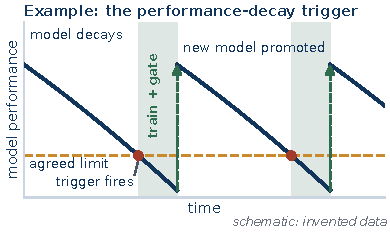
\includegraphics[width=6.6cm]{images/class27_triggers.pdf}};
\foreach \y/\ico/\ttl/\txt in {0/calendar-alt/Schedule/{A fixed cadence: nightly, weekly.}, -0.8/database/Data volume/{Enough new labeled data accumulated.}, -1.6/wave-square/Drift signal/{A Class 33 detector raises an alert.}, -2.4/chart-line/Performance decay/{A tracked metric crosses a set limit.}, -3.2/hand-pointer/Manual request/{A person asks for a run, with a reason.}} {
  \node[tile, fill=white, draw=courseblue!55, thick, anchor=north west, minimum width=6.5cm, minimum height=0.7cm] at (6.9,\y) {};
  \node[circle, fill=courseblue, text=white, minimum size=0.46cm, inner sep=0, font=\scriptsize] at (7.3,\y-0.35) {\faIcon{\ico}};
  \node[anchor=west, font=\scriptsize\bfseries, text=courseblue, inner sep=0pt] at (7.7,\y-0.2) {\ttl};
  \node[anchor=west, font=\scriptsize, text width=5.5cm, align=left, inner sep=0pt] at (7.7,\y-0.5) {\txt};
}
\keyidea{-4.15}{Any trigger starts the same pipeline. The evaluation gate, not the trigger, decides whether the new model is used.}
\end{tikzpicture}
\coursefooter
\end{cframe}

\begin{cframe}{Anatomy of a continuous training pipeline}{\cterm{Pipeline}{an ordered set of automated steps, each consuming the output of the one before.}\cterm{Gate}{an explicit pass-or-fail check that decides whether a run may continue.}\cterm{Champion}{the model currently in use, against which candidates are compared.}}
\centering
\begin{tikzpicture}
\foreach \i/\ico/\ttl/\sub/\col in {0/play-circle/Trigger/{schedule, event, or request}/courseblue, 1/check-double/Validate data/{schema, freshness, volume}/courseblue, 2/cogs/Train candidate/{same code, new data}/courseblue, 3/balance-scale/Evaluate vs champion/{frozen held-out set}/courseblue, 4/flag-checkered/Promote or reject/{register and release, or discard}/coursegold} {
  \pgfmathsetmacro{\x}{\i*2.825}
  \node[rounded corners=4pt, fill=\col, text=white, anchor=north west, minimum width=2.1cm, minimum height=1.7cm, text width=1.9cm, align=center, font=\scriptsize\bfseries] (s\i) at (\x,0) {\faIcon{\ico}\\[2pt]\ttl\\[2pt]{\tiny\mdseries\sub}};
}
\foreach \i/\j in {0/1,1/2,2/3,3/4} {\draw[arrowgray] (s\i.east) -- (s\j.west);}
\foreach \i in {0,1,2,3} {
  \pgfmathsetmacro{\gx}{2.4625+\i*2.825}
  \draw[arrowred] (\gx,-1.15) -- (\gx,-2.25);
  \node[circle, fill=coursegold, draw=white, line width=1.5pt, text=white, minimum size=0.55cm, inner sep=0, font=\scriptsize] at (\gx,-0.85) {\faIcon{shield-alt}};
}
\node[tilered, anchor=north west, minimum width=13.4cm, minimum height=0.65cm, text width=12.9cm, align=left, font=\scriptsize] at (0,-2.3) {{\bfseries\color{coursered}\faIcon{hand-paper}\ A failed gate stops the run.} The reason is logged and the current champion keeps serving; nothing is promoted by default.};
\keyidea{-3.3}{Every arrow is a gate: a candidate that fails a stage should not move forward automatically.}
\end{tikzpicture}
\coursefooter
\end{cframe}

\begin{cframe}{Data validation before training}{\cterm{Label distribution}{how often each outcome class appears in the training data.}\cterm{Freshness}{how recent the newest data is, compared with what the pipeline assumes.}}
\centering
\begin{tikzpicture}
\infotile{0}{0}{4.3}{2.5}{tileblue}{courseblue}{table}{Schema checks}{Are the expected columns present, with the expected types?\\[4pt]{\itshape Catches: a renamed column.}}
\infotile{4.55}{0}{4.3}{2.5}{tileblue}{courseblue}{clock}{Freshness checks}{Is the data as recent as the trigger assumed?\\[4pt]{\itshape Catches: a stale extract reused by mistake.}}
\infotile{9.1}{0}{4.3}{2.5}{tileblue}{courseblue}{balance-scale}{Volume and balance}{Is there enough signal, and is the label distribution sane?\\[4pt]{\itshape Catches: almost no examples of the rare class.}}
\warning{-2.8}{exclamation-triangle}{Why it comes first.}{A pipeline that trains on broken data just automates producing a broken model faster.}
\end{tikzpicture}
\coursefooter
\end{cframe}

\begin{cframe}{Evaluation gates before promotion}{\cterm{Held-out set}{data kept aside during training and used only to evaluate.}\cterm{Business metric}{a measure tied to operational cost or benefit, such as the false-alert rate.}}
\centering
\begin{tikzpicture}
\node[tileblue, anchor=north west, minimum width=3.9cm, minimum height=1.2cm, text width=3.5cm, align=left] at (0,0) {{\bfseries\color{courseblue}\faIcon{medal}\ Champion}\\[2pt]{\scriptsize the model in use today}};
\node[tilegray, anchor=north west, minimum width=3.9cm, minimum height=1.2cm, text width=3.5cm, align=left] at (4.75,0) {{\bfseries\color{coursegray}\faIcon{lock}\ Frozen held-out set}\\[2pt]{\scriptsize same data for both models}};
\node[tilegold, anchor=north west, minimum width=3.9cm, minimum height=1.2cm, text width=3.5cm, align=left] at (9.5,0) {{\bfseries\goldink\faIcon{seedling}\ Candidate}\\[2pt]{\scriptsize the newly trained model}};
\draw[arrowgray] (3.9,-0.6) -- (4.75,-0.6);
\draw[arrowgray] (9.5,-0.6) -- (8.65,-0.6);
\node[tileblue, anchor=north west, minimum width=6.6cm, minimum height=1.15cm, text width=6.2cm, align=left, font=\scriptsize] at (0,-1.45) {{\bfseries\color{courseblue}\faIcon{chart-bar}\ STATISTICAL METRIC}\\How well does it predict on the held-out set?};
\node[tilegold, anchor=north west, minimum width=6.6cm, minimum height=1.15cm, text width=6.2cm, align=left, font=\scriptsize] at (6.8,-1.45) {{\bfseries\goldink\faIcon{coins}\ BUSINESS METRIC}\\What does it cost or save: review load, false alerts, missed detections?};
\node[tilegreen, anchor=north west, minimum width=4.3cm, minimum height=1.4cm, text width=3.9cm, align=left, font=\scriptsize] at (0,-2.85) {{\bfseries\color{coursegreen}\faIcon{check-circle}\ Better on every metric}\\Promote the candidate.};
\node[tilegold, anchor=north west, minimum width=4.3cm, minimum height=1.4cm, text width=3.9cm, align=left, font=\scriptsize] at (4.55,-2.85) {{\bfseries\goldink\faIcon{user-check}\ Mixed result}\\Better on one metric, worse on another: a human decides, no automatic merge.};
\node[tilered, anchor=north west, minimum width=4.3cm, minimum height=1.4cm, text width=3.9cm, align=left, font=\scriptsize] at (9.1,-2.85) {{\bfseries\color{coursered}\faIcon{times-circle}\ Not better}\\Reject it; the champion keeps serving.};
\end{tikzpicture}
\coursefooter
\end{cframe}

\begin{cframe}{Champion-challenger extends into training}{\cterm{Challenger}{a candidate model under evaluation against the champion.}\cterm{Shadow evaluation}{running a candidate on live requests without using its answers.}}
\centering
\begin{tikzpicture}
\node[tile, fill=courseice, anchor=north west, minimum width=2.6cm, minimum height=1.1cm, font=\footnotesize\bfseries, text=courseblue] at (0,-1.45) {\faIcon{stream}\ Live requests};
\node[tileblue, anchor=north west, minimum width=3.8cm, minimum height=1.1cm, text width=3.4cm, align=left] at (4.4,0) {{\bfseries\color{courseblue}\faIcon{medal}\ Champion}\\[2pt]{\scriptsize serves every request}};
\node[tilegold, dashed, anchor=north west, minimum width=3.8cm, minimum height=1.1cm, text width=3.4cm, align=left] at (4.4,-2.9) {{\bfseries\goldink\faIcon{seedling}\ Challenger}\\[2pt]{\scriptsize sees a copy of the traffic}};
\draw[arrowgray] (2.6,-1.75) -- (4.4,-0.55);
\draw[arrowgold, dashed] (2.6,-2.25) -- (4.4,-3.45);
\node[font=\tiny\bfseries, text=coursegold!65!black, fill=white, inner sep=1pt] at (3.5,-2.85) {COPY};
\node[tilegreen, anchor=north west, minimum width=4.0cm, minimum height=1.1cm, text width=3.6cm, align=left, font=\scriptsize] at (9.4,0) {{\bfseries\color{coursegreen}\faIcon{check}\ Answers used}\\returned to users};
\node[tilegray, anchor=north west, minimum width=4.0cm, minimum height=1.1cm, text width=3.6cm, align=left, font=\scriptsize] at (9.4,-2.9) {{\bfseries\color{coursegray}\faIcon{ban}\ Answers not used}\\only logged for comparison};
\draw[arrowgray] (8.2,-0.55) -- (9.4,-0.55);
\draw[arrowgold, dashed] (8.2,-3.45) -- (9.4,-3.45);
\node[tilegold, anchor=north west, minimum width=4.0cm, minimum height=1.1cm, text width=3.6cm, align=left, font=\scriptsize] at (9.4,-1.5) {{\bfseries\goldink\faIcon{balance-scale}\ Compare}\\same requests; promote only if it wins};
\draw[arrowgray] (11.4,-1.1) -- (11.4,-1.5);
\draw[arrowgray] (11.4,-2.9) -- (11.4,-2.6);
\keyidea{-4.2}{Shadow evaluation on live traffic catches problems that offline metrics miss, before the challenger serves anyone.}
\end{tikzpicture}
\coursefooter
\end{cframe}

\begin{cframe}{Where continuous training meets CI/CD}{\cterm{Cron trigger}{a time-based rule, such as every night at 02:00, that starts a workflow.}\cterm{Workflow}{a defined sequence of automated jobs, started by a trigger.}}
\centering
\begin{tikzpicture}
\node[chip, fill=courseblue, anchor=north west, minimum width=2.3cm, minimum height=0.6cm, font=\scriptsize\bfseries] at (0,0) {\faIcon{server}\ SERVING};
\foreach \k/\t in {0/Commit, 1/Test, 2/Package, 3/Deploy} {
  \node[tileblue, anchor=north west, minimum width=1.9cm, minimum height=0.6cm, font=\scriptsize\bfseries, text=courseblue] at ({2.5+2.1*\k},0) {\t};
}
\foreach \k in {0,1,2} {\draw[arrowgray] ({4.4+2.1*\k},-0.3) -- ({4.6+2.1*\k},-0.3);}
\node[chip, fill=coursegreen, anchor=north west, minimum width=2.3cm, minimum height=0.6cm, font=\scriptsize\bfseries] at (0,-1.3) {\faIcon{redo-alt}\ TRAINING};
\foreach \k/\t in {0/Trigger, 1/Validate, 2/Train, 3/Evaluate, 4/Register} {
  \node[tilegreen, anchor=north west, minimum width=1.9cm, minimum height=0.6cm, font=\scriptsize\bfseries, text=courseblue] at ({2.5+2.1*\k},-1.3) {\t};
}
\foreach \k in {0,1,2,3} {\draw[arrowgray] ({4.4+2.1*\k},-1.6) -- ({4.6+2.1*\k},-1.6);}
\node[tilegold, anchor=north west, minimum width=13.4cm, minimum height=0.8cm, text width=12.6cm, align=left, font=\footnotesize] at (0,-2.4) {{\bfseries\goldink\faIcon{layer-group}\ Same discipline on both paths.} Version it, test it, package it, and review it: training code is code.};
\callout{-3.45}{clock}{Building block.}{Class 32's GitHub Actions cron trigger is a small but real way to start exactly this kind of scheduled job.}
\end{tikzpicture}
\coursefooter
\end{cframe}

\begin{cframe}{Failure modes and governance of automated retraining}{\cterm{Feedback loop}{a cycle in which a model's outputs influence the data it later learns from.}\cterm{Drift masking}{hiding a real change by retraining on data that already contains it.}\cterm{Audit trail}{a record that lets a third person reconstruct what happened and why.}}
\centering
\begin{tikzpicture}
\node[anchor=west, font=\tiny\bfseries, text=coursered] at (0,0.15) {FOUR WAYS IT GOES WRONG};
\infotile{0}{0}{3.95}{1.95}{tilered}{coursered}{sync-alt}{Feedback loops}{A fraud model's blocking decisions can bias its later labels.}
\infotile{4.1}{0}{3.95}{1.95}{tilered}{coursered}{theater-masks}{Drift masking}{Retraining can bake a temporary anomaly in as if it were normal.}
\infotile{0}{-2.05}{3.95}{1.95}{tilered}{coursered}{random}{Silent schema drift}{An upstream field changes meaning and nobody updates the training code.}
\infotile{4.1}{-2.05}{3.95}{1.95}{tilered}{coursered}{robot}{Unbounded automation}{A bad candidate is promoted because a gate is missing or weak.}
\node[anchor=west, font=\tiny\bfseries, text=courseblue] at (8.4,0.15) {HOW A TEAM KEEPS IT GOVERNED};
\foreach \y/\ico/\ttl/\txt in {0/clipboard-list/Log every run/{Trigger, data snapshot, metrics, and the decision.}, -1.3/user-check/A person in the loop/{Human approval for high-stakes promotions.}, -2.6/code-branch/Version it together/{Code and data references go with the model.}} {
  \node[tileblue, anchor=north west, minimum width=5.0cm, minimum height=1.15cm] at (8.4,\y) {};
  \badge{8.95}{\y-0.58}{courseblue}{\ico}
  \node[anchor=west, font=\scriptsize\bfseries, text=courseblue, text width=3.4cm, align=left, inner sep=0pt] at (9.5,\y-0.3) {\ttl};
  \node[anchor=north west, text width=3.5cm, align=left, font=\scriptsize, inner sep=0pt] at (9.5,\y-0.5) {\txt};
}
\warning{-4.15}{ban}{Rule.}{Every automated stage needs an explicit condition for stopping, not just for proceeding.}
\end{tikzpicture}
\coursefooter
\end{cframe}

% ================================================================== PART 4
\sectiondivider{4}{Repository}{folder-open}{continuous training automates the train-and-retrain box; what does this repository already contain?}{$\bullet$\ How the repository illustrates MLOps\\[3pt]$\bullet$\ Practical Component: an honest gap\\[3pt]$\bullet$\ A discussion question on automation and judgment}

\begin{cframe}{How this repository illustrates MLOps}{\cterm{Operationalization}{turning an experiment into something that is run, supported, and monitored.}\cterm{Submodule}{a Git repository embedded inside another repository and tracked at a fixed version.}}
\centering
\begin{tikzpicture}
\node[anchor=west, font=\tiny\bfseries, text=coursegray] at (0,0.15) {WHERE TO LOOK};
\node[anchor=west, font=\tiny\bfseries, text=coursegold!65!black] at (4.75,0.15) {WHAT IT SHOWS};
\node[anchor=west, font=\tiny\bfseries, text=coursegray] at (11.25,0.15) {CLOSEST STAGE};
\reporow{-0.3}{notebooks/}{Early-stage exploration and model building.}{coursered}{Early}
\reporow{-1.12}{pasteurization/, streamlit/}{Behavior becomes a service or an interface.}{coursegold}{Emerging}
\reporow{-1.94}{tutorials/\{Docker, GitHubActions, Jenkins\}}{Operationalization paths: packaging, automation, and delivery.}{coursegold}{Emerging}
\reporow{-2.76}{App\_Stream.py}{Monitoring that connects deployed behavior to feedback and drift response.}{courseblue}{Managed}
\node[tilered, anchor=north west, minimum width=13.4cm, minimum height=1.1cm, text width=12.8cm, align=left, font=\scriptsize] at (0,-3.65) {{\bfseries\color{coursered}\faIcon{exclamation-triangle}\ Practical Component: an honest gap.} There is currently no automated retraining pipeline: the training code (notebooks, \texttt{streamlit/modeling.py}) and the cron workflow (\texttt{tutorials/GitHubActions}) are not wired together. Closing the gap is suggested as a separate project, for example a GitHub submodule; this class stays conceptual on purpose.};
\end{tikzpicture}
\coursefooter
\end{cframe}

\begin{cframe}{Discussion prompt}{\cterm{Human in the loop}{a design in which a person must review or approve an automated decision.}}
\centering
\begin{tikzpicture}
\node[tilegold, anchor=north west, minimum width=13.4cm, minimum height=1.9cm] at (0,0) {};
\badge{0.75}{-0.95}{coursegold}{comments}
\node[anchor=west, text width=11.4cm, align=left] at (1.5,-0.95) {{\bfseries\tiny\goldink QUESTION}\\[3pt]{\bfseries\large\color{courseblue}If a retraining pipeline ran fully unattended, which single gate would you refuse to automate away, and why?}};
\infotile{0}{-2.15}{6.6}{1.75}{tileblue}{courseblue}{balance-scale}{Why this question}{It forces a concrete stance on where human judgment stays load-bearing.}
\infotile{6.8}{-2.15}{6.6}{1.75}{tileblue}{courseblue}{history}{Where it returns}{The governance theme comes back in the monitoring and scaling discussion of Class 33.}
\end{tikzpicture}
\coursefooter
\end{cframe}

% ------------------------------------------------------------------ closing
\section{Wrap-up}\gdef\currentsectionname{Wrap-up}
\begin{frame}{From this class to the next}
\centering
\begin{tikzpicture}
\foreach \i/\lab/\bg/\fg in {1/Problem/courseice/coursegray, 2/Data/courseice/coursegray, 3/Features/courseice/coursegray, 4/Model/courseice/coursegray, 5/Interface/courseice/coursegray, 6/Delivery/courseblue/white, 7/Monitor/courseblue/white, 8/Evolution/courseblue/white} {
  \node[rounded corners=3pt, minimum width=1.55cm, minimum height=0.6cm, font=\scriptsize\bfseries, fill=\bg, text=\fg] at ({0.78+(\i-1)*1.68},0) {\lab};
}
\node[font=\tiny\bfseries, text=courseblue] at (6.7,-0.52) {THIS CLASS PUTS DELIVERY, MONITORING, AND EVOLUTION UNDER ONE LIFECYCLE};
\foreach \x/\sty/\ico/\ttl/\txt in {0/tileblue/lightbulb/What stays with us/{$\bullet$\ MLOps: one lifecycle, from experiment to monitoring.\\[3pt]$\bullet$\ Maturity: repeatability, observability, clear roles.\\[3pt]$\bullet$\ Gates matter more than automation.}, 4.55/tileblue/project-diagram/Use it in your project/{$\bullet$\ Judge whether your project is an engineered system.\\[3pt]$\bullet$\ Say what would trigger a retraining run and what would stop a bad candidate.}, 9.1/tilegold/arrow-right/Next: Class 28/{\textbf{Pasteurization Challenge, Session 2.}\\[3pt]Your thin slice is validated and a change request tests it. Class 29: online learning and concept drift.}} {
  \node[\sty, anchor=north west, minimum width=4.3cm, minimum height=3.8cm] at (\x,-0.95) {};
  \badge{\x+0.65}{-1.6}{courseblue}{\ico}
  \node[anchor=west, text width=3.0cm, align=left, font=\small\bfseries, text=courseblue] at (\x+1.2,-1.6) {\ttl};
  \node[anchor=north west, text width=3.9cm, align=left, font=\scriptsize] at (\x+0.2,-2.25) {\txt};
}
\node[tilegold, fill=white, anchor=north west, minimum width=13.4cm, minimum height=0.95cm, text width=12.6cm, align=left, font=\footnotesize] at (0,-5.0) {{\bfseries\goldink\faIcon{route}\ Course thread.} Training and delivery are two automatable paths that need the same gates and versioning.};
\end{tikzpicture}
\coursefooter
\end{frame}

% ------------------------------------------------------------------ references
\begin{frame}{Papers and materials}
\centering
\begin{tikzpicture}
\node[chip, anchor=west, minimum width=3.4cm, minimum height=0.68cm, font=\scriptsize\bfseries, align=left] at (0,-0.5) {\faIcon{file-alt}\ Papers};
\node[anchor=west, text width=9.8cm, font=\scriptsize, align=left] at (3.6,-0.5) {Sculley, D. et al. (2015). \href{https://research.google/pubs/pub46555/}{Hidden Technical Debt in Machine Learning Systems}. NeurIPS.};
\draw[courseice!70!courseblue, line width=0.5pt] (0,-1.0) -- (13.4,-1.0);
\node[chip, anchor=west, minimum width=3.4cm, minimum height=0.68cm, font=\scriptsize\bfseries, align=left] at (0,-1.7) {\faIcon{book}\ Books};
\node[anchor=west, text width=9.8cm, font=\scriptsize, align=left] at (3.6,-1.7) {\href{https://www.oreilly.com/library/view/practical-mlops/9781098103002/}{Practical MLOps}. O'Reilly.\\Huyen, C. \href{https://www.oreilly.com/library/view/designing-machine-learning/9781098107956/}{Designing Machine Learning Systems}. O'Reilly.};
\draw[courseice!70!courseblue, line width=0.5pt] (0,-2.4) -- (13.4,-2.4);
\node[chip, anchor=west, minimum width=3.4cm, minimum height=0.68cm, font=\scriptsize\bfseries, align=left] at (0,-3.2) {\faIcon{cloud}\ Guides};
\node[anchor=west, text width=9.8cm, font=\scriptsize, align=left] at (3.6,-3.2) {\href{https://cloud.google.com/architecture/mlops-continuous-delivery-and-automation-pipelines-in-machine-learning}{Google Cloud: MLOps, continuous delivery and automation pipelines (CI/CD/CT)}.\\\href{https://neptune.ai/blog/mlops-best-practices}{MLOps best practices overview}.\\\href{https://evidentlyai.com/ml-observability}{ML observability materials from Evidently}.};
\draw[courseice!70!courseblue, line width=0.5pt] (0,-4.0) -- (13.4,-4.0);
\end{tikzpicture}
\coursefooter
\end{frame}

\end{document}
